\chapter{Volatilidad Local Estocástica}
Como se ha visto en el capítulo anterior, una de las principales limitaciones del modelo de Black--Scholes es que la hipótesis de volatilidad constante impide reproducir la sonrisa y la superficie de volatilidad implícita observadas en mercado.\medskip 

Esta limitación motiva la introducción de modelos más flexibles, capaces de incorporar una volatilidad dependiente del estado del mercado o de evolucionar de forma aleatoria en el tiempo. Entre las extensiones más utilizadas se encuentran los modelos de volatilidad local y los modelos de volatilidad estocástica. Sin embargo, considerados por separado, cada uno de estos enfoques presenta ciertas restricciones. Con el objetivo de combinar sus principales ventajas, se introducen los modelos de Volatilidad Local Estocástica, conocidos como modelos \textit{Stochastic--Local Volatility}(SLV).\medskip

En este capítulo introducimos primero los modelos de volatilidad local y de volatilidad estocástica, prestando especial atención al modelo de Heston. A continuación se presenta el modelo híbrido Heston--SLV, que será el enfoque utilizado posteriormente en la comparación con la metodología de Entropía Relativa Mínima. El desarrollo sigue principalmente la notación de \cite{DanielArrietaPresentation} y el tratamiento de Heston--SLV de \cite{oosterlee2021modelos}.

\section{Volatilidad local}

En esta sección se introduce el modelo de volatilidad local, conocido habitualmente como modelo LV por sus siglas en inglés, \textit{Local Volatility }. \medskip

El concepto de volatilidad local fue introducido por Dupire en \cite{Dupire1994} como una forma de incorporar la dependencia de la volatilidad respecto del strike y del vencimiento. La idea principal consiste en sustituir el parámetro constante $\sigma_{\text{imp}}$ del modelo de Black--Scholes por una función determinista que depende del tiempo y del nivel del subyacente. De este modo, bajo la medida neutral al riesgo $\mathbb{Q}$, la dinámica del precio del activo se modeliza mediante la ecuación diferencial estocástica

\[
dS(t) = rS(t)\,dt + \sigma_{\mathrm{LV}}(S(t),t)S(t)\,dW(t),
\]

con condición inicial \(S(t_0)=S_0\), donde \(r\) representa el tipo de interés libre de riesgo, \(W(t)\) es un movimiento browniano y \(\sigma_{\mathrm{LV}}(S,t)\) es la función de volatilidad local evaluada a lo largo de la trayectoria.\medskip

El objetivo del modelo es escoger la función $\sigma_{\mathrm{LV}}(S,t)$ de forma que los precios de opciones europeas generados por la dinámica anterior sean consistentes con los precios observados en el mercado. 

Por otra parte, suponiendo ausencia de arbitraje, el valor de la opción \(V(S,t)\) verifica la EDP
\begin{equation}
\label{eq:edp_volatilidad_local}
   \begin{cases}
    \frac{\partial V}{\partial t} + \frac{1}{2}\sigma^2_{\mathrm{LV}}(S,t) S^2 \frac{\partial^2 V}{\partial S^2} + r S \frac{\partial V}{\partial S} - rV = 0, \\
    V(S,T) = \max\{S-K,0\}. 
\end{cases} 
\end{equation}

La ecuación \ref{eq:edp_volatilidad_local} es una ecuación en derivadas parciales de Kolmogorov hacia atrás, que describe cómo el valor de la opción \(V(S,t)\) evoluciona a lo largo del tiempo. Sin embargo, para obtener una expresión explícita de la función \(\sigma_{\mathrm{LV}}\) en términos de precios de mercado resulta más conveniente trabajar con la ecuación forward asociada a la densidad del subyacente. \medskip

Recordemos el siguiente resultado, que relaciona una ecuación diferencial estocástica general con la evolución temporal de su densidad de transición.

\begin{theorem}[Ecuación de Fokker--Planck]
Sea $S(t)$ un proceso estocástico definido por la ecuación diferencial estocástica
\[
dS(t)=\bar{\mu}(S(t),t)\,dt+\bar{\sigma}(S(t),t)\,dW(t),
\qquad S(t_0)=S_0,
\]
para $t_0\leq t\leq T$. Entonces, la densidad de transición
\[
f_{S(t)}(y)\equiv f_{S(t)}(y;t_0,S_0)
\]
asociada al proceso $S(t)$ satisface la ecuación forward de Kolmogorov, también conocida como ecuación de Fokker--Planck,
\begin{equation}
\begin{cases}
\dfrac{\partial f_{S(t)}(y)}{\partial t}
+\dfrac{\partial}{\partial y}\left[\bar{\mu}(t,y)f_{S(t)}(y)\right]
-\dfrac{1}{2}\dfrac{\partial^2}{\partial y^2}
\left[\bar{\sigma}^2(t,y)f_{S(t)}(y)\right]=0, \\[0.3cm]
f_{S(t_0)}(y)=\delta(y-S_0).
\end{cases}
\label{eq:fokker_planck}
\end{equation}
\end{theorem}

Una demostración de este resultado se puede encontrar en \cite[Cap.~5, Secs.~5.1 y 5.7, pp.~283 y 368--369]{Karatzas1991}. El modelo de volatilidad local se basa precisamente en esta ecuación forward. En efecto, bajo la medida neutral al riesgo, la dinámica del subyacente en el modelo de volatilidad local viene dada por
\begin{equation}
dS(t)=rS(t)\,dt+\sigma_{\mathrm{LV}}(S,t)S(t)\,dW(t),
\qquad S(t_0)=S_0.
\label{eq:dinamica_local_vol}
\end{equation}
Comparando \ref{eq:dinamica_local_vol} con la ecuación diferencial estocástica general del teorema anterior, se tiene
\[
\bar{\mu}(t,y)=ry,
\qquad
\bar{\sigma}(t,y)=y\sigma_{\mathrm{LV}}(y,t).
\]
Por tanto, la ecuación de Fokker--Planck asociada a la dinámica de volatilidad local es
\begin{equation}
\frac{\partial f_{S(t)}(y)}{\partial t}
+
\frac{\partial}{\partial y}\left[ry f_{S(t)}(y)\right]
-
\frac{1}{2}
\frac{\partial^2}{\partial y^2}
\left[
y^2\sigma_{\mathrm{LV}}^2(y,t) f_{S(t)}(y)
\right]
=0.
\label{eq:fokker_planck_local_vol}
\end{equation}

Por otra parte, por el resultado establecido por Breeden y Litzenberger en \cite{BreedenPrices}, la densidad neutral al riesgo del precio del subyacente está directamente relacionada con las cotizaciones de mercado de opciones europeas. En concreto, la fórmula de Breeden--Litzenberger establece que
\begin{equation}
\label{eq:Breeden--Litzenberger}
\frac{\partial^2 V_c(K,T)}{\partial K^2}
=
e^{-r(T-t_0)} f_{S(T)}(K),
\end{equation}
donde $V_c(K,T)$ denota el precio, observado en el instante inicial $t_0$, de una opción call europea con strike $K$ y vencimiento $T$. Equivalentemente,
\[
f_{S(T)}(K)
=
e^{r(T-t_0)}
\frac{\partial^2 V_c(K,T)}{\partial K^2}.
\]
Por tanto, la densidad neutral al riesgo del precio del subyacente en el vencimiento $T$ puede obtenerse, al menos formalmente, a partir de la segunda derivada del precio de las opciones call respecto del strike.

Hay que tener en cuenta, sin embargo, que en el mercado solo se cotiza un número limitado de opciones para una acción concreta. Por ello, resulta difícil extraer con precisión la densidad neutral al riesgo a partir de esas pocas cotizaciones de mercado. En términos teóricos, para recuperar dicha densidad de forma exacta sería necesario disponer de un continuo de precios de opciones para todos los strikes $K\in[0,\infty)$.\medskip

A continuación, se puede utilizar la ecuación de Fokker--Planck junto con la relación de Breeden--Litzenberger para obtener la expresión de la volatilidad local. Para ello, partimos del precio de una call europea escrito en términos de la densidad neutral al riesgo:
\begin{equation}
V_c(K,T)
=
e^{-r(T-t_0)}
\int_K^{\infty} (y-K) f_{S(T)}(y)\,dy.
\label{eq:call_density}
\end{equation}
Derivando \ref{eq:call_density} respecto de $K$, se obtiene
\[
\frac{\partial V_c(K,T)}{\partial K}
=
-e^{-r(T-t_0)}
\int_K^{\infty} f_{S(T)}(y)\,dy,
\]
y derivando de nuevo respecto de $K$,
\[
\frac{\partial^2 V_c(K,T)}{\partial K^2}
=
e^{-r(T-t_0)}f_{S(T)}(K),
\]
que coincide con la fórmula de Breeden--Litzenberger.

Ahora derivamos \ref{eq:call_density} respecto del vencimiento \(T\). Usando la ecuación de Fokker--Planck asociada a la dinámica \ref{eq:dinamica_local_vol}, e integrando por partes, se obtiene
\begin{equation}
\frac{\partial V_c(K,T)}{\partial T}
=
-rK\frac{\partial V_c(K,T)}{\partial K}
+
\frac{1}{2}K^2\sigma_{\mathrm{LV}}^2(K,T)
\frac{\partial^2 V_c(K,T)}{\partial K^2}.
\label{eq:dupire_intermediate}
\end{equation}
Reordenando la igualdad anterior, llegamos a la expresión de la varianza local:
\begin{equation}
\label{eq:Dupire_local_vol}
\sigma_{\mathrm{LV}}^2(K,T)
=
\frac{
\dfrac{\partial V_c(K,T)}{\partial T}
+
rK\dfrac{\partial V_c(K,T)}{\partial K}
}{
\dfrac{1}{2}K^2
\dfrac{\partial^2 V_c(K,T)}{\partial K^2}
}.
\end{equation}

Esta fórmula muestra que la función de volatilidad local \(\sigma_{\mathrm{LV}}(K,T)\) queda caracterizada a partir de la superficie de precios de opciones europeas observada en el mercado. En consecuencia, el modelo de volatilidad local puede ajustarse exactamente a las cotizaciones de opciones europeas, sin necesidad de introducir un procedimiento de calibración paramétrica. En la práctica, no obstante, las derivadas parciales que aparecen en \ref{eq:Dupire_local_vol} deben aproximarse numéricamente a partir de un conjunto finito de precios de mercado, lo que puede generar inestabilidades, especialmente en zonas donde la densidad neutral al riesgo es pequeña. \medskip

De forma equivalente, si se trabaja directamente con una superficie suficientemente regular de volatilidad implícita \(\widehat{\sigma}(t,K)\), se puede escribir la fórmula de Dupire en términos de la varianza total. Para ello, se introduce
\[
w(t,K)=t\widehat{\sigma}^2(t,K),
\]
donde \(t\) representa el vencimiento y \(K\) el strike. Definiendo
\[
y=\log\left(\frac{K}{S_0e^{rt}}\right),
\]
la varianza local puede expresarse como
\begin{equation}
\label{eq:varianza_local_implicita}
\sigma_{\mathrm{LV}}^2(K,t)=
\frac{
\dfrac{\partial w}{\partial t}
+
rK\dfrac{\partial w}{\partial K}
}{
1
+
K\dfrac{\partial w}{\partial K}
\left(\frac{1}{2}-\frac{y}{w}\right)
+
\frac{1}{2}K^2\dfrac{\partial^2 w}{\partial K^2}
+
\frac{1}{2}K^2\left(\dfrac{\partial w}{\partial K}\right)^2
\left(
-\frac{1}{8}
-\frac{1}{2w}
+
\frac{y^2}{2w^2}
\right)
}.
\end{equation}
Esta formulación es útil cuando la entrada principal es la superficie de volatilidad implícita. En la implementación, no obstante, se utiliza la forma equivalente basada en precios: primero se transforma la superficie implícita en una superficie de precios call \(V_c(K,T)\) mediante Black--Scholes y después se aplica \ref{eq:Dupire_local_vol}.\medskip
%%%%%%%%%%%%%%%%%%%%%%%%%%%%%%%%%%%%%%%%%%%%%%%%%%%%%%%%%%%%%%%%%%%%%%%%

\subsection{Simulación del modelo LV}

Una vez obtenida la función de volatilidad local, el modelo puede simularse directamente a partir de la dinámica definida en \ref{eq:dinamica_local_vol}. A diferencia del modelo de Black--Scholes, en el que la volatilidad es constante, en el modelo LV la volatilidad debe evaluarse en cada instante temporal y en cada nivel alcanzado por el subyacente. Es decir, a lo largo de cada trayectoria se utiliza el valor
\[
\sigma_{\mathrm{LV}}(S(t_i),t_i).
\]

El punto delicado del método es la regularidad de la superficie utilizada. Si la superficie de precios no es suficientemente suave, la aproximación de \(\partial_T V_c\), \(\partial_K V_c\) y \(\partial_{KK}V_c\) puede producir valores inestables de \(\sigma_{\mathrm{LV}}\), especialmente en zonas donde la densidad neutral al riesgo es pequeña. Por este motivo, la construcción de una superficie coherente es esencial para obtener una volatilidad local estable.

Una vez calculada la función \(\sigma_{\mathrm{LV}}(t,K)\), las trayectorias del subyacente se generan mediante un esquema de Euler explícito. Dada una partición temporal
\[
0=t_0<t_1<\cdots<t_N=T,
\qquad \Delta t=t_{i+1}-t_i,
\]
la discretización viene dada por
\begin{equation}
\label{eq:euler_local_vol}
S(t_{i+1})
=
S(t_i)
+
rS(t_i)\Delta t
+
\sigma_{\mathrm{LV}}(t_i,S(t_i))S(t_i)\sqrt{\Delta t}\,Z_i,
\qquad
Z_i\sim N(0,1).
\end{equation}

En la expresión anterior, aunque la volatilidad local se haya obtenido inicialmente como función del vencimiento y del strike, durante la simulación se evalúa en el nivel alcanzado por el subyacente. Es decir, en cada paso temporal se toma formalmente
\[
K=S(t_i),
\]
de modo que la volatilidad aplicada en la trayectoria es \(\sigma_{\mathrm{LV}}(S(t_i),t_i)\).\medskip

La principal ventaja del modelo LV es que, al estar construido a partir de la superficie de volatilidad implícita de mercado, permite reproducir de forma precisa los precios de opciones europeas vainilla observados inicialmente. Sin embargo, al tratarse de una volatilidad determinista dependiente del nivel del subyacente y del tiempo, no incorpora una dinámica estocástica propia para la evolución futura de la volatilidad. Esta limitación será el punto de partida de la siguiente sección.
%%%%%%%%%%%%%%%%%%%%%%%%%%%%%%%%%%%%%%%%%%%%%%%%%%%%%%%%%%%%%%%%%%%%%%%%%%%%%%%%%%%%%%%%%%%%%%%%%%%%%%%%%%%%%%%%%%%%%%%%%%%
\section{Volatilidad estocástica}

Como se ha visto en la sección anterior, los modelos de volatilidad local permiten ajustar de forma precisa una superficie de volatilidad implícita observada en un instante inicial. Sin embargo, esta ventaja también constituye una de sus principales limitaciones: la dinámica queda construida a partir de una superficie concreta de mercado y no incorpora de forma explícita una fuente aleatoria propia para la evolución futura de la volatilidad. Esto puede ser suficiente para la valoración de opciones europeas, pero resulta más restrictivo cuando se consideran productos dependientes de la trayectoria o sensibles a la evolución futura de la sonrisa de volatilidad, como ocurre con las opciones \textit{forward-start}. \medskip

Una forma natural de superar esta limitación consiste en modelar la volatilidad, o la varianza instantánea, mediante un proceso estocástico propio. Esta idea da lugar a los modelos de volatilidad estocástica, conocidos habitualmente como modelos SV, por sus siglas en inglés, \textit{Stochastic Volatility}. En este tipo de modelos, la aleatoriedad del mercado no procede únicamente del movimiento del activo subyacente, sino también de la evolución de su volatilidad. Entre los modelos clásicos de esta familia se encuentran los trabajos de Hull y White, Stein y Stein, Heston, y Schöbel y Zhu. \medskip

En esta sección nos centraremos en el modelo de Heston, que será el modelo de volatilidad estocástica utilizado posteriormente como base para construir el modelo híbrido Heston--SLV. Antes de introducirlo, conviene presentar brevemente el proceso CIR, ya que la varianza en el modelo de Heston sigue precisamente una dinámica de este tipo.

\subsection{El proceso CIR}

El proceso de Cox--Ingersoll--Ross, o proceso CIR, fue introducido originalmente en el contexto de modelos de tipos de interés. En el modelo de Heston, este proceso se utiliza para describir la evolución de la varianza instantánea del activo subyacente. Su dinámica viene dada por
\begin{equation}
\label{eq:cir_process}
dv(t)=\kappa(\theta-v(t))\,dt+\gamma\sqrt{v(t)}\,dW(t),
\qquad v(t_0)=v_0>0.
\end{equation}

El parámetro \(\kappa>0\) representa la velocidad de reversión a la media, \(\theta>0\) es el nivel medio de largo plazo y \(\gamma>0\) mide la intensidad de las fluctuaciones aleatorias del proceso. 

Una característica fundamental del proceso CIR es la presencia del término $\sqrt{v(t)}$ en la parte difusiva. Este término hace que la volatilidad instantánea del propio proceso disminuya cuando $v(t)$ se aproxima a cero, evitando que la varianza tome valores negativos. Bajo la condición de Feller,
\begin{equation}
\label{eq:feller_condition}
2\kappa\theta\geq \gamma^2,
\end{equation}
el proceso permanece estrictamente positivo. Si esta condición no se cumple, el proceso sigue siendo no negativo, pero puede acercarse al origen e incluso alcanzarlo. En tal caso, el comportamiento numérico cerca de cero requiere especial cuidado. \medskip

Esta propiedad justifica su uso para modelizar la varianza instantánea en Heston y, posteriormente, en Heston--SLV. Para estudiar de forma más precisa el efecto de la condición de Feller, puede utilizarse la distribución de transición exacta del proceso CIR. Si $s<t$ y se condiciona al valor inicial $v(s)$, entonces la variable $v(t) \mid v(s)$ puede expresarse en términos de una distribución chi-cuadrado no central:
\[
v(t) \mid v(s)
\sim
c_{s,t}\,\chi'^2_d(\lambda_{s,t}),
\]
donde
\[
c_{s,t}
=
\frac{\gamma^2}{4\kappa}
\left(1-e^{-\kappa(t-s)}\right),
\qquad
d=
\frac{4\kappa\theta}{\gamma^2},
\]
y
\[
\lambda_{s,t}
=
\frac{
4\kappa e^{-\kappa(t-s)}v(s)
}{
\gamma^2\left(1-e^{-\kappa(t-s)}\right)
}.
\]
Por tanto, la densidad de transición del proceso CIR viene dada por
\[
f_{v(t)\mid v(s)}(x)
=
\frac{1}{c_{s,t}}\,
f_{\chi'^2_d(\lambda_{s,t})}
\left(\frac{x}{c_{s,t}}\right),
\qquad x>0.
\]

Para ilustrar el efecto de la condición de Feller, en la Figura \ref{fig:cir_feller_density} se representa la densidad de transición del proceso CIR en dos situaciones: una en la que la condición se satisface y otra en la que no se satisface. En ambos casos se toman los siguientes parámetros:
\[
s=0,\qquad t=2,\qquad v(s)=0.04,\qquad \theta=0.04,
\qquad \kappa=1.5,
\]
y se modifica únicamente el parámetro $\gamma$. Para $\gamma=0.2$ se obtiene
\[
q_F
=
\frac{2\kappa\theta}{\gamma^2}-1
=
2.0000,
\]
por lo que la condición de Feller se satisface. En cambio, para $\gamma=0.5$ se obtiene
\[
q_F=-0.5200,
\]
de modo que la condición de Feller no se cumple. 

\begin{figure}[H]
\centering
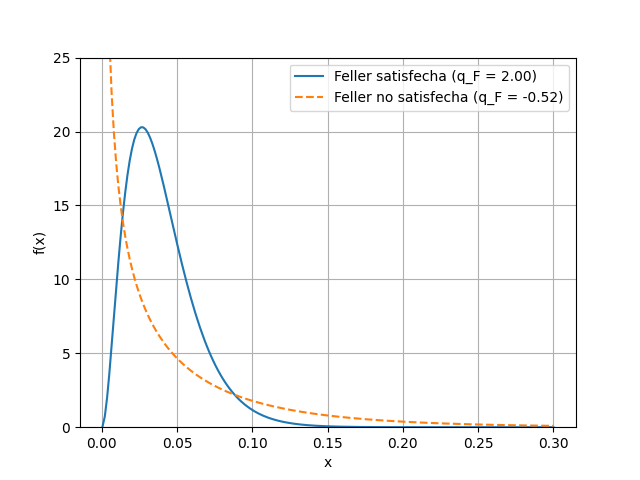
\includegraphics[width=0.8\textwidth]{cir_feller_density.png}
\caption{Función de densidad de probabilidad para $\gamma=0.2$ (condición satisfecha) y $\gamma=0.5$ (condición no satisfecha).}
\label{fig:cir_feller_density}
\end{figure}
Cuando se satisface la condición de Feller, la densidad queda concentrada en valores positivos y la probabilidad de que el proceso se acerque al origen es reducida. En cambio, cuando la condición no se cumple, la densidad presenta mayor masa cerca de cero, por lo que la varianza puede tomar valores muy pequeños. Este comportamiento es relevante en el modelo de Heston, y posteriormente en el modelo Heston--SLV, ya que el proceso CIR se utiliza para describir la varianza instantánea del subyacente.

\subsection{El modelo de Heston}

El modelo de Heston es uno de los modelos de volatilidad estocástica más utilizados en finanzas cuantitativas. Su principal idea consiste en sustituir la volatilidad constante del modelo de Black--Scholes por una varianza instantánea aleatoria que sigue un proceso CIR. Bajo la medida neutral al riesgo $\mathbb{Q}$, el modelo viene dado por el sistema de ecuaciones diferenciales estocásticas
\begin{equation}
\label{eq:heston_sv}
\begin{cases}
dS(t) = rS(t)\,dt+\sqrt{v(t)}S(t)\,dW^{S,\mathbb{Q}}(t), \\[0.15cm]
dv(t) = \kappa(\theta-v(t))\,dt+\gamma\sqrt{v(t)}\,dW^{v,\mathbb{Q}}(t),
\end{cases}
\end{equation}
con condiciones iniciales
\[
S(t_0)=S_0>0,
\qquad
v(t_0)=v_0>0.
\]

Los movimientos brownianos que aparecen en \ref{eq:heston_sv} están correlados según
\begin{equation}
\label{eq:heston_correlation}
dW^{S,\mathbb{Q}}(t)\,dW^{v,\mathbb{Q}}(t)=\rho_{S,v}\,dt.
\end{equation}

La primera ecuación describe la evolución del activo subyacente. Como estamos trabajando bajo la medida neutral al riesgo, la deriva del activo es el tipo libre de riesgo $r$. \medskip

La segunda ecuación describe la evolución de la varianza instantánea. Como se ha indicado, esta varianza sigue un proceso CIR, de modo que revierte hacia el nivel medio \(\theta\) con velocidad \(\kappa\) y presenta fluctuaciones aleatorias controladas por el parámetro \(\gamma\), conocido como volatilidad de la volatilidad. \medskip

\begin{observation}[Cambio de medida]
La formulación anterior se ha escrito directamente bajo la medida neutral al riesgo \(\mathbb{Q}\), ya que el objetivo del trabajo es la valoración de derivados y la calibración a precios de mercado. Esto es coherente con el marco introducido en el capítulo anterior: cuando se toma como numerario la cuenta bancaria libre de riesgo, la medida de valoración asociada es la medida neutral al riesgo, bajo la cual el precio descontado del activo debe ser una martingala.\medskip

En el modelo de Black--Scholes, el paso de la medida histórica \(\mathbb{P}\) a la medida neutral al riesgo \(\mathbb{Q}\) consiste, de forma esencial, en sustituir la deriva real \(\mu\) del activo por el tipo libre de riesgo \(r\):
\[
dS(t)=\mu S(t)\,dt+\sigma S(t)\,dW^{\mathbb{P}}(t),
\qquad
dS(t)=rS(t)\,dt+\sigma S(t)\,dW^{\mathbb{Q}}(t).
\]
En el modelo de Heston la idea es análoga, aunque más delicada, puesto que existen dos fuentes de aleatoriedad: una asociada al subyacente y otra asociada a la varianza.\medskip

Bajo la medida $\mathbb{P}$, la varianza podría escribirse con parámetros propios de la dinámica real del mercado. Sin embargo, al pasar a la medida de valoración, dichos parámetros pueden verse modificados por el cambio de medida. Por ello, en la práctica el modelo de Heston suele formularse directamente bajo \(\mathbb{Q}\), entendiendo que
\[
\kappa,\qquad \theta,\qquad \gamma,\qquad \rho_{S,v},\qquad v_0
\]
son parámetros de valoración calibrados a precios de opciones.
\end{observation}

\subsubsection{Ecuación de valoración de Heston}

Sea \(V(t,S,v)\) el valor de un derivado europeo escrito sobre el activo \(S\), suponiendo que la dinámica del par \((S(t),v(t))\) viene dada por el modelo de Heston. La ecuación de valoración asociada puede obtenerse mediante dos enfoques equivalentes: el enfoque de martingala y el enfoque de cobertura. Ambos procedimientos se desarrollan en \cite[pp.~245--247]{oosterlee2021modelos}; aquí se recoge únicamente la ecuación resultante, ya que la deducción sigue las mismas ideas introducidas para el modelo de Black--Scholes. \medskip

Desde el punto de vista de martingala, el valor descontado del derivado debe satisfacer
\begin{equation}
\label{eq:heston_expectation}
\frac{V(t,S(t),v(t))}{N(t)}
=
\mathbb{E}^{\mathbb{Q}}
\left[
\left.
\frac{V(T,S(T),v(T))}{N(T)}
\right|
\mathcal{F}_t
\right],
\end{equation}
donde \(N(t)\) representa la cuenta bancaria libre de riesgo. Si el tipo de interés \(r\) es constante, entonces \(N(t)=e^{rt}\), y la expresión anterior puede escribirse como
\[
V(t,S(t),v(t))
=
e^{-r(T-t)}
\mathbb{E}^{\mathbb{Q}}
\left[
V(T,S(T),v(T))
\mid
\mathcal{F}_t
\right].
\]

En particular, para un derivado europeo con payoff \(\Phi(S(T))\), se tiene la condición terminal
\[
V(T,S,v)=\Phi(S).
\]
Aplicando el lema de Itô bidimensional a \(V(t,S(t),v(t))\) y usando las dinámicas de \ref{eq:heston_sv}, se obtiene la siguiente ecuación en derivadas parciales:
\begin{equation}
\label{eq:heston_edp}
\frac{\partial V}{\partial t}
+rS\frac{\partial V}{\partial S}
+\kappa(\theta-v)\frac{\partial V}{\partial v}
+\frac{1}{2}vS^2\frac{\partial^2 V}{\partial S^2}
+\rho_{S,v}\gamma vS\frac{\partial^2 V}{\partial S\partial v}
+\frac{1}{2}\gamma^2v\frac{\partial^2 V}{\partial v^2}
-rV=0.
\end{equation}

El enfoque de cobertura conduce a la misma ecuación, aunque la construcción de la cartera replicante es más compleja que en Black--Scholes. En este caso existen dos fuentes de riesgo, una asociada al subyacente \(S(t)\) y otra asociada a la varianza \(v(t)\). Por tanto, si solo se negocian el activo subyacente y la cuenta bancaria, el mercado no permite cubrir directamente ambas fuentes de incertidumbre. Para completar la cobertura sería necesario incorporar algún instrumento adicional sensible a la volatilidad. Esta observación refleja la relación entre los modelos de volatilidad estocástica y la incompletitud de mercado. \medskip

La ecuación \ref{eq:heston_edp} también admite una interpretación probabilística mediante Feynman--Kac, que expresa el precio como una esperanza descontada bajo la medida neutral al riesgo. Además, una de las principales ventajas del modelo de Heston es que pertenece a la clase de modelos afines. Esto permite obtener su función característica en forma semianalítica, lo que facilita la valoración eficiente de opciones europeas y la posterior calibración del modelo a superficies de volatilidad implícita, por ejemplo mediante métodos basados en Fourier como el método COS.

\subsubsection*{Limitaciones del modelo de Heston}

El modelo de Heston introduce una fuente estocástica para la varianza y, por tanto, permite generar sonrisas y skews de volatilidad implícita que no pueden reproducirse en el modelo de Black--Scholes con volatilidad constante. Además, sus parámetros tienen una interpretación financiera clara: la correlación \(\rho_{S,v}\) influye principalmente en la inclinación del skew, la volatilidad de la volatilidad \(\gamma\) afecta a la curvatura de la sonrisa, \(v_0\) determina el nivel inicial de varianza, \(\theta\) representa el nivel de largo plazo y \(\kappa\) controla la velocidad de reversión hacia dicho nivel.

Sin embargo, aunque esta estructura proporciona una dinámica más rica que la de un modelo de volatilidad local puro, el modelo de Heston no garantiza por sí solo un ajuste exacto a toda la superficie de volatilidad implícita observada en mercado. En la práctica, la calibración se realiza escogiendo los parámetros
\[
\kappa,\qquad \theta,\qquad \gamma,\qquad \rho_{S,v},\qquad v_0
\]
de forma que los precios generados por el modelo se aproximen lo mejor posible a los precios de opciones cotizadas. No obstante, al tratarse de un modelo paramétrico con un número reducido de parámetros, puede no ser suficientemente flexible para reproducir con precisión todas las estructuras observadas en la superficie, especialmente cuando se consideran varios vencimientos y strikes.

Por tanto, el modelo de Heston presenta una ventaja importante frente a la volatilidad local: incorpora una dinámica estocástica de la varianza, lo que resulta especialmente relevante para productos sensibles a la evolución futura de la volatilidad. Sin embargo, también presenta una limitación: su capacidad de ajuste a la superficie inicial puede ser menor que la de un modelo de volatilidad local. Esta tensión entre ajuste inicial y dinámica futura motiva la introducción de los modelos de volatilidad local estocástica, que combinan una componente local, destinada a reproducir la superficie de mercado, con una componente estocástica, encargada de modelar la evolución aleatoria de la volatilidad.

%%%%%%%%%%%%%%%%%%%%%%%%%%%%%%%%%%%%%%%%%%%%%%%%%%%%%%%%%%%%%%%%%%%%%%%%%%%%%%%%%%%%%%%%

\section{Modelo de volatilidad local estocástica}

Los modelos de volatilidad local estocástica, conocidos como modelos \textit{Stochastic--Local Volatility} o SLV, combinan las ideas introducidas en las secciones anteriores. Por un lado, incorporan una componente local que permite ajustar la superficie de volatilidad implícita observada en mercado. Por otro lado, mantienen una componente estocástica para describir de forma más realista la evolución futura de la volatilidad.\medskip

Esta combinación permite corregir algunas de las limitaciones de los modelos LV y SV considerados por separado, y resulta especialmente útil en productos sensibles a la dinámica futura de la sonrisa de volatilidad, como las opciones \textit{forward-start}. En esta sección se introduce la formulación general del modelo SLV y, posteriormente, su particularización al caso Heston--SLV.

\subsection{Formulación general del modelo SLV}

Bajo la medida neutral al riesgo \(\mathbb{Q}\), un modelo de volatilidad local estocástica puede escribirse de forma general como
\begin{equation}
\label{eq:general_slv}
\begin{cases}
\dfrac{dS(t)}{S(t)}
=
r\,dt+\eta(S(t),t)\,\xi(v(t))\,dW^S(t), \\[0.25cm]
dv(t)
=
a_v(v(t),t)\,dt+b_v(v(t),t)\,dW^v(t), \\[0.25cm]
dW^S(t)\,dW^v(t)=\rho_{S,v}\,dt.
\end{cases}
\end{equation}

En esta formulación, \(S(t)\) representa el precio del activo subyacente y \(v(t)\) es el factor estocástico asociado a la volatilidad. La función \(\eta(S(t),t)\) representa la componente local del modelo, también denominada función de apalancamiento (leverage function).\medskip

Por otro lado, la función \(\xi(v(t))\) introduce la dependencia respecto del factor estocástico \(v(t)\), mientras que las funciones \(a_v\) y \(b_v\) determinan, respectivamente, la deriva y la difusión de dicho proceso. Finalmente, el parámetro \(\rho_{S,v}\in[-1,1]\) mide la correlación instantánea entre las dos fuentes de aleatoriedad.\medskip

El modelo \ref{eq:general_slv} contiene como casos particulares algunos de los modelos estudiados anteriormente. Si se toma \(\eta(S,t)=1\), se recupera un modelo puramente de volatilidad estocástica. En cambio, si la componente estocástica no introduce aleatoriedad adicional y se identifica el producto \(\eta(S,t)\xi(v(t))\) con la volatilidad local \(\sigma_{\mathrm{LV}}(S,t)\), se obtiene el modelo de volatilidad local.\medskip

Por tanto, el modelo SLV puede interpretarse como una extensión híbrida que combina la capacidad de ajuste de los modelos de volatilidad local con la dinámica de los modelos de volatilidad estocástica. En la siguiente subsección se estudia cómo se determina la componente local \(\eta\), que es el elemento que permite conectar ambas partes del modelo.

\subsection{Componente de volatilidad local del modelo}

El elemento que conecta la parte local y la parte estocástica del modelo SLV es la función \(\eta(S,t)\). Esta función se introduce para que el modelo reproduzca la superficie de volatilidad implícita observada en mercado, manteniendo al mismo tiempo una dinámica estocástica para la volatilidad.\medskip

La determinación de la función \(\eta\) se basa en la relación de consistencia entre el modelo SLV y el modelo de volatilidad local asociado a la superficie de mercado. Esta relación, conocida habitualmente como condición de proyección (Markovian projection), puede encontrarse en \cite[Sec.~10.2.1]{oosterlee2021modelos}. En particular, se impone que la varianza instantánea efectiva del modelo SLV, condicionada al nivel del subyacente, coincida con la varianza local obtenida mediante la fórmula de Dupire. Por tanto,
\begin{equation}
\label{eq:slv_projection}
\sigma_{\mathrm{LV}}^2(K,t)
=
\eta^2(K,t)\,
\mathbb{E}^{\mathbb{Q}}
\left[
\xi^2(v(t))\mid S(t)=K
\right].
\end{equation}

A partir de \ref{eq:slv_projection}, la componente local del modelo queda determinada por
\begin{equation}
\label{eq:eta_slv_general}
\eta(K,t)
=
\frac{
\sigma_{\mathrm{LV}}(K,t)
}{
\sqrt{
\mathbb{E}^{\mathbb{Q}}
\left[
\xi^2(v(t))\mid S(t)=K
\right]
}
}.
\end{equation}

En esta expresión, el numerador \(\sigma_{\mathrm{LV}}(K,t)\) es la función de volatilidad local introducida en la sección de volatilidad local. Por tanto, la componente local del modelo SLV hereda la información contenida en los precios de opciones vainilla observados inicialmente. \medskip

El papel de la función \(\eta\) no es sustituir a \(\sigma_{\mathrm{LV}}\), sino adaptar la componente estocástica del modelo para que, al condicionar por el nivel del subyacente, la varianza efectiva del modelo SLV coincida con la varianza local. De esta forma, la relación \ref{eq:slv_projection} permite combinar el ajuste inicial proporcionado por el modelo LV con la dinámica estocástica introducida por el proceso \(v(t)\).

El denominador, en cambio, depende de la componente estocástica del modelo. Concretamente, recoge el valor esperado de \(\xi^2(v(t))\) condicionado a que el subyacente tome el valor \(K\) en el instante \(t\). Este término no se conoce, en general, de forma explícita, ya que depende de la distribución conjunta de \((S(t),v(t))\) bajo el propio modelo SLV. Por ello, debe aproximarse numéricamente.

Una forma habitual de estimar esta esperanza condicional es mediante un procedimiento no paramétrico basado en simulaciones Monte Carlo. Para un instante temporal \(t_i\), se dispone de un conjunto de trayectorias simuladas
\[
\left(S_{j}(t_i),v_{j}(t_i)\right),
\qquad j=1,\ldots,N.
\]
Las trayectorias se agrupan según el valor alcanzado por el subyacente \(S_j(t_i)\), dividiendo el rango de valores simulados en intervalos o bins. Si \(I_k\) denota el \(k\)-ésimo bin y \(J_k=\{m:S_m(t_i)\in I_k\}\) es el conjunto de índices de las trayectorias que caen en dicho bin, entonces, para una trayectoria \(j\in J_k\), se aproxima
\begin{equation}
\label{eq:conditional_expectation_bins_general}
\mathbb{E}^{\mathbb{Q}}
\left[
\xi^2(v(t_i))\mid S(t_i)=S_{j}(t_i)
\right]
\approx
\frac{1}{N_k}
\sum_{m\in J_k}
\xi^2\left(v^{(m)}(t_i)\right),
\end{equation}
donde \(N_k\) es el número de trayectorias contenidas en dicho bin.

Así, para cada instante temporal y para cada nivel simulado del subyacente, la función \(\eta\) se calcula como el cociente entre la volatilidad local de mercado y la raíz cuadrada de la esperanza condicional estimada. En consecuencia, \(\eta\) actúa como un corrector local de la componente estocástica: ajusta el modelo para reproducir las volatilidades vainilla observadas, pero sin eliminar la aleatoriedad introducida por el proceso \(v(t)\).

\subsection{Modelo Heston--SLV}

En este trabajo se considera una particularización del modelo SLV en la que la componente estocástica de la volatilidad viene dada por el modelo de Heston. Es decir, se toma como factor estocástico la varianza instantánea \(v(t)\), cuya dinámica sigue un proceso CIR. En la formulación general \ref{eq:general_slv}, esto equivale a tomar
\[
\xi(v(t))=\sqrt{v(t)},
\qquad
a_v(v(t),t)=\kappa(\theta-v(t)),
\qquad
b_v(v(t),t)=\gamma\sqrt{v(t)}.
\]

Sustituyendo estas expresiones en el modelo SLV general, se obtiene el modelo Heston--SLV bajo la medida neutral al riesgo \(\mathbb{Q}\),
\begin{equation}
\label{eq:heston_slv}
\begin{cases}
\dfrac{dS(t)}{S(t)}
=
r\,dt+\eta(S(t),t)\sqrt{v(t)}\,dW^S(t), \\[0.25cm]
dv(t)
=
\kappa(\theta-v(t))\,dt+\gamma\sqrt{v(t)}\,dW^v(t), \\[0.25cm]
dW^S(t)\,dW^v(t)=\rho_{S,v}\,dt.
\end{cases}
\end{equation}

La primera ecuación describe la evolución del activo subyacente. La segunda ecuación coincide con la dinámica de la varianza en el modelo de Heston \ref{eq:heston_sv}. El parámetro \(\kappa\) representa la velocidad de reversión a la media, \(\theta\) el nivel medio de largo plazo, \(\gamma\) la volatilidad de la volatilidad y \(\rho_{S,v}\) la correlación instantánea entre el movimiento del subyacente y el de la varianza.

En este caso, como \(\xi^2(v(t))=v(t)\), la relación general para la componente local se simplifica a
\begin{equation}
\label{eq:heston_slv_leverage}
\eta(K,t)
=
\frac{
\sigma_{\mathrm{LV}}(K,t)
}{
\sqrt{
\mathbb{E}^{\mathbb{Q}}
\left[
v(t)\mid S(t)=K
\right]
}
}.
\end{equation}

Esta expresión muestra la estructura híbrida del modelo. El numerador \(\sigma_{\mathrm{LV}}(K,t)\) procede de la superficie de volatilidad local obtenida mediante Dupire y recoge la información de mercado contenida en las opciones vainilla. El denominador incorpora la información generada por la dinámica estocástica de Heston, a través de la esperanza condicional de la varianza dado el nivel del subyacente.

Por tanto, el modelo Heston--SLV puede interpretarse como una corrección local del modelo de Heston. La componente estocástica proporciona una dinámica más realista para la evolución futura de la volatilidad, mientras que la función \(\eta\) ajusta dicha dinámica para que sea consistente con la superficie de volatilidad implícita observada inicialmente. A continuación, describimos cómo se simula numéricamente este modelo mediante Monte Carlo.

\subsection{Simulación Monte Carlo del modelo}

La simulación del modelo Heston--SLV se realiza mediante un método de Monte Carlo. Para ello, se considera una partición uniforme del intervalo temporal \([0,T]\),
\[
0=t_0<t_1<\cdots<t_m=T,
\qquad
\Delta t=\frac{T}{m},
\]
y se simulan \(N\) trayectorias del par \((S(t),v(t))\). Denotaremos por
\[
S_{i,j}\approx S(t_j),
\qquad
v_{i,j}\approx v(t_j),
\]
el valor del subyacente y de la varianza en la trayectoria \(i\), con \(i=1,\ldots,N\), y en el instante \(t_j\), con \(j=0,\ldots,m\).

En cada instante temporal es necesario calcular la función de apalancamiento
\[
\eta(S_{i,j},t_j)
=
\frac{
\sigma_{\mathrm{LV}}(S_{i,j},t_j)
}{
\sqrt{
\mathbb{E}^{\mathbb{Q}}
\left[
v(t_j)\mid S(t_j)=S_{i,j}
\right]
}
}.
\]
El numerador \(\sigma_{\mathrm{LV}}(S_{i,j},t_j)\) procede de la superficie de volatilidad local obtenida mediante Dupire. El denominador, en cambio, depende de la distribución conjunta de \((S(t),v(t))\) bajo el modelo Heston--SLV y, en general, no se conoce de forma explícita.
%%%%%%%%%%%%
En cada instante \(t_j\), se aproxima la esperanza condicional mediante el estimador por bins descrito en \ref{eq:conditional_expectation_bins_general} y definimos
\[
\widehat{E}_{i,j}
=
\frac{1}{N_k^{(j)}}
\sum_{\ell\in J_k^{(j)}} v_{\ell,j}.
\]

Para introducir la correlación entre el movimiento del subyacente y el de la varianza, se generan dos variables normales estándar independientes,
\[
X_{i,j},Y_{i,j}\sim N(0,1).
\]
La fuente de aleatoriedad asociada al subyacente viene dada por \(X_{i,j}\), mientras que la correspondiente a la varianza se construye como
\[
\rho_{S,v}X_{i,j}
+
\sqrt{1-\rho_{S,v}^2}\,Y_{i,j}.
\]
De esta forma, ambas fuentes de aleatoriedad tienen correlación \(\rho_{S,v}\).

Aplicando un esquema de Euler a la dinámica Heston--SLV, se obtiene
\begin{equation}
\label{eq:euler_heston_slv_S}
S_{i,j+1}
=
S_{i,j}
+
rS_{i,j}\Delta t
+
\eta(S_{i,j},t_j)\sqrt{v_{i,j}}\,S_{i,j}\sqrt{\Delta t}\,X_{i,j},
\end{equation}
y
\begin{equation}
\label{eq:euler_heston_slv_v}
v_{i,j+1}
=
v_{i,j}
+
\kappa(\theta-v_{i,j})\Delta t
+
\gamma\sqrt{v_{i,j}}\sqrt{\Delta t}
\left(
\rho_{S,v}X_{i,j}
+
\sqrt{1-\rho_{S,v}^2}\,Y_{i,j}
\right).
\end{equation}

Sustituyendo la expresión discreta de \(\eta\), la ecuación del subyacente puede escribirse también como
\begin{equation}
\label{eq:euler_heston_slv_S_expanded}
S_{i,j+1}
=
S_{i,j}
+
rS_{i,j}\Delta t
+
\sqrt{
\frac{
\sigma_{\mathrm{LV}}^2(S_{i,j},t_j)
}{
\widehat{E}_{i,j}
}
}
S_{i,j}\sqrt{v_{i,j}}\sqrt{\Delta t}\,X_{i,j}.
\end{equation}
Esta forma muestra explícitamente cómo intervienen las dos componentes del modelo: la volatilidad local \(\sigma_{\mathrm{LV}}\), asociada a la superficie de mercado, y la esperanza condicional \(\widehat{E}_{i,j}\), asociada a la dinámica estocástica de la varianza.

Aunque el esquema anterior puede escribirse de forma aditiva para \(S_{i,j}\), también es habitual utilizar una versión exponencial del esquema. En ella, los coeficientes se evalúan al inicio de cada intervalo temporal y se mantienen constantes durante el paso \([t_j,t_{j+1}]\). Es decir, durante ese intervalo se toman como dados los valores
\[
\eta(S_{i,j},t_j),
\qquad
v_{i,j},
\qquad
r.
\]
Bajo esta aproximación, la actualización del subyacente viene dada por
\begin{equation}
\label{eq:log_euler_heston_slv}
S_{i,j+1}
=
S_{i,j}
\exp\left[
\left(
r-\frac{1}{2}\eta^2(S_{i,j},t_j)v_{i,j}
\right)\Delta t
+
\eta(S_{i,j},t_j)\sqrt{v_{i,j}}\sqrt{\Delta t}\,X_{i,j}
\right].
\end{equation}
Esta forma mantiene la positividad del subyacente y resulta natural para una dinámica de tipo lognormal con coeficientes constantes en cada paso temporal.\medskip

Además del esquema de Euler, se ha considerado también un esquema de tipo Almost Exact Simulation (AES), siguiendo el enfoque descrito en \cite[Sec.~10.2.3]{oosterlee2021modelos}. Este tipo de métodos busca reducir el sesgo de discretización asociado a la simulación del modelo Heston--SLV, especialmente en la componente de varianza y en la estimación de la esperanza condicional que aparece en la función de apalancamiento. Los detalles concretos de la implementación numérica y de los esquemas considerados se discutirán posteriormente.\medskip


Desde el punto de vista numérico, la simulación del proceso de varianza requiere cierto cuidado, ya que el proceso CIR debe permanecer no negativo. El tratamiento concreto utilizado para evitar valores negativos de la varianza se detallará posteriormente en la sección de implementación numérica.\medskip

Con esto queda definido el modelo Heston--SLV que se utilizará en el resto del trabajo. La construcción anterior muestra cómo se combinan la información de mercado recogida por la volatilidad local y la dinámica estocástica de la varianza propia del modelo de Heston. La valoración concreta de opciones vainilla y opciones de tipo \textit{forward-start} mediante las trayectorias simuladas se presentará más adelante, dentro del capítulo de implementación numérica, para poder compararla de forma directa con la valoración obtenida mediante Entropía Relativa Mínima.
